%\documentclass[handout]{beamer}
\documentclass{beamer}

\usepackage[english]{babel}
\usepackage[latin1]{inputenc}
\usepackage{textpos}
\usepackage{epstopdf}
\epstopdfsetup{update}
%\usepackage{pgfpages}
%\pgfpagesuselayout{resize to}[letterpaper,landscape]
%\usepackage{epstopdf}
%\epstopdfsetup{update}
\usepackage{pgfplots}
\usepackage{pgfbaseimage}
\usepackage{amsmath} 						%More mathematical
\usepackage{multirow}
%\usepackage[absolute,overlay]{textpos}
%\usepackage[tikz]{bclogo}
%\usepackage{etoolbox}
% listings for matlab code:
\usepackage{listings}
%\usepackage[autolinebreaks, useliterate]{mcode}
\lstset{backgroundcolor=\color[gray]{0.9}}

\usepackage{chemplants}
\usepackage{cancel}
\usepackage{graphicx}
\usetikzlibrary{math}
\usepackage{wasysym}
\usepackage{marvosym}

\usetikzlibrary{shapes.arrows}
\tikzset{My Arrow Style/.style={single arrow, draw=green!40!gray, very thick, fill=green!20!gray!10, anchor=base, align=center,text width=2cm,text=green!40!gray,rotate=-90,minimum width=0.5cm, inner sep=1mm, minimum height=0.5cm}}
\newcommand{\MyArrow}[2][]{\tikz[baseline] \node [My Arrow Style,#1] {#2};}

%-------------------------------------------------
% FOOTER
%
% Choose your footer style, by commenting other options:
%
%% - Clean: no footer, except of page number
\mode<presentation>{\usetheme{presentationTemplateBiomathFClean}}
%%  - Info: a fixed footer with basic presenter information
%\mode<presentation>{\usetheme{presentationTemplateBiomathFInfo}}
%%  - Section: Provide the sections and current section in the footer 
%\mode<presentation>{\usetheme{presentationTemplateBiomathFSection}}
%-------------------------------------------------


%voor de hand-outs
%\usepackage{pgfpages}
%\pgfpagesuselayout{2 on 1}[a4paper,border shrink=5mm]

\title{\LARGE Modelling and Simulation \normalsize of Biosystems}
\title{Modelling and Simulation of Biosystems}
\author[Daniel Illana]{Daniel Illana Gonz\'alez} %(daniel.illanagonzalez@ugent.be)}
\subtitle{Project session -- general guidelines \& suggestions}
\date{Academic year 2024-2025}


\newcommand{\mtx}[2]
  {\left[\begin{array}{#1}#2\end{array}\right]}
\newcommand{\eqset}[1]
  {\left\{\begin{array}{rcl}#1\end{array}\right.}
\newcommand{\rbar}[2]
  {\left.#1\right|_{#2}}
\newcommand{\atwp}[1]
  {\rbar{#1}{\overline{X},\overline{U}}}

\usepackage{mdframed}

\newenvironment{opgave}[2][]{%
	\mdfsetup{%
		frametitle={%
			\tikz[baseline=(current bounding box.east),outer sep=0pt]
			\node[anchor=east,rectangle,fill=gray!40]
			{\strut #1};}%
	}
	\mdfsetup{%
		innertopmargin=10pt,linecolor=white!30,%
		linewidth=0pt,topline=true,%
		frametitleaboveskip=\dimexpr-\ht\strutbox\relax%
	}
	
	\begin{mdframed}[]\relax}{%
\end{mdframed}}


% Table of contents at the beginning of each section
%\AtBeginSection[]
%{
%  \begin{frame}
%    \frametitle{Outline}
%    \tableofcontents[currentsection]
%  \end{frame}
%}

% Title page customisation
\titlegraphic{}

\begin{document}

\frame[plain]{\titlepage}

%%%%%%%%%%%%%%%%%%%%%%%%%%%%%%%%%%%%%%%%%%%%%%%%%%%%%%%%%%%%%%%%%%
%%%%%%%%%%%%%%%%%%%%%%%%%%%%%%%%%%%%%%%%%%%%%%%%%%%%%%%%%%%%%%%%%%
%% Project assignment
%%%%%%%%%%%%%%%%%%%%%%%%%%%%%%%%%%%%%%%%%%%%%%%%%%%%%%%%%%%%%%%%%%
%%%%%%%%%%%%%%%%%%%%%%%%%%%%%%%%%%%%%%%%%%%%%%%%%%%%%%%%%%%%%%%%%%

\frame{
\begin{center}
\Huge \textbf{Project assignment}
\end{center}
}

\frame{
	\frametitle{Assignment}
See {\color{ugent-la}\texttt{project.pdf}} assignment in Ufora.
\vspace*{0.5cm}

\begin{itemize}
\item Apply Modsim principles to a \textit{small}, self-contained example \vfill
%\item Inspiration $\Rightarrow$ one of our abstracts \vfill
\item In a Pluto notebook environment (cf. {\color{ugent-la}\texttt{project\_template.jl}}) \vfill
\item Eight to ten pages when printed (Export... $\rightarrow$ HTML/PDF) \vfill
\item Contains the following: \vfill
	\begin{itemize}
	\item context, relevancy, summary, conclusion \vfill
	\item model based on differential equations or probabilistic model \vfill
	\item clear outline of variables and parameters \vfill
	\item include: optimization, calibration, deeper insight gain, uncertainty assessment, sensitivity analysis, stochasticity... \vfill 
	\end{itemize}
\item Check also {\color{ugent-la}Grading rubric} and {\color{ugent-la}``Tips and advice''} in Ufora. \vfill
\item You can find some project examples in Ufora and our website.
\end{itemize}
}	

\frame{
\frametitle{Typical procedure}

\begin{figure}[hbt]
  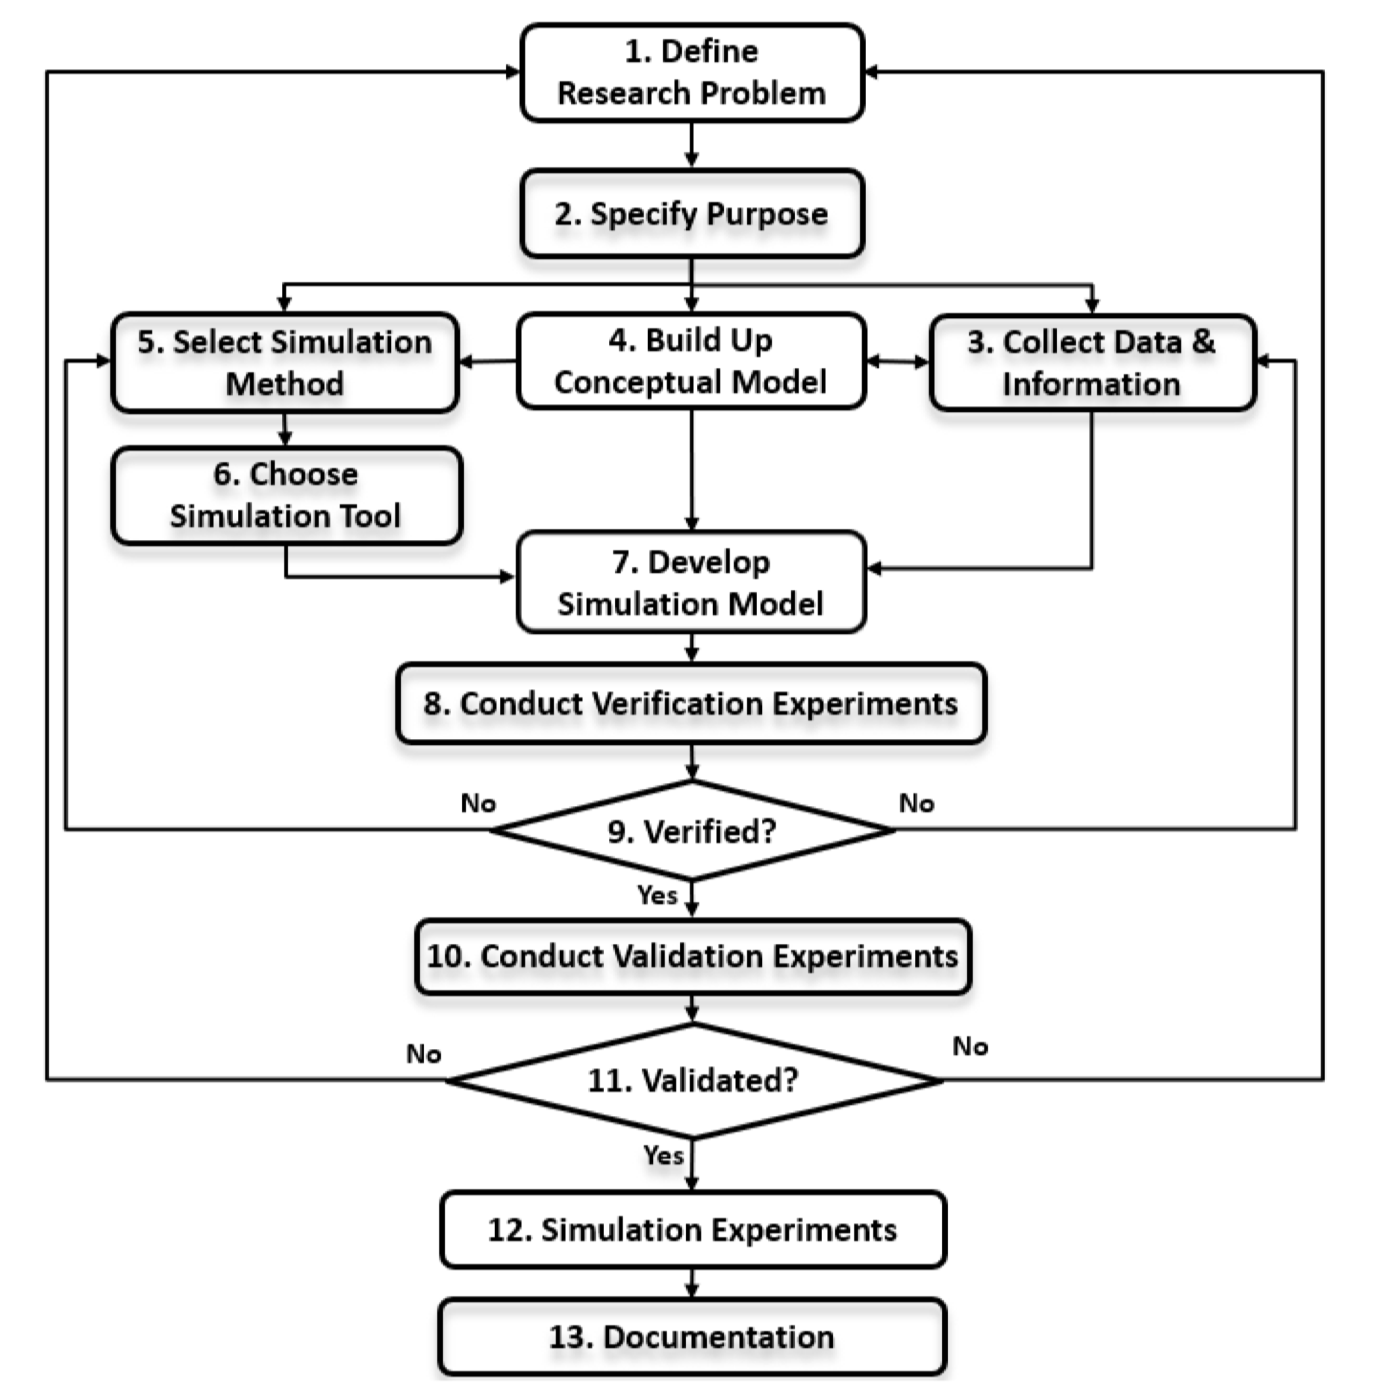
\includegraphics[width=0.7\linewidth]{figs/diagram.png}
\end{figure}
}

\frame{
\frametitle{Solving problems using modeling and simulation}

\bigskip

\begin{block}{Problem solving}
Decide how to \textbf{simplify the problem} while still capturing all essential elements: all steps in the problem-solving process are equally important!
\end{block} \medskip \pause

%\setbeamercolor{itemize/enumerate body}{fg=gray}
\begin{enumerate}[<+->]
	\item \textbf{Formulate problem and model} \smallskip
	\begin{itemize}
		\item List objectives or goals, requirements, assumptions and limitations \smallskip
		\item Problem description: system states, inputs, outputs and parameters \smallskip
		\item A system can be regarded as a hierarchy of less complex subsystems
	\end{itemize} \medskip

	\item \textbf{Implement system model}: start simple, then add complexity \medskip
	\item \textbf{Conduct simulation experiments}: e.g., sensitivity analysis\medskip
	\item \textbf{Interpret results}: what did we learn from the experiments? \medskip
	\item \textbf{Document study}: \textit{if it's not written down, it didn't happen} \medskip
	\item \textbf{Implement conclusions}: what  impact/influence will it have? \medskip
	\item \textbf{Validate model}: are the model and analyzed data accurate?
\end{enumerate}
}

\frame{
\frametitle{Guidelines}

Some more guidelines:

\begin{itemize}[<+->]
	\item Define clear/achievable goals to keep in mind during the whole project. Develop a common understanding of the project goals.
	\item Allocate \textit{sufficient} time: meet regularly with all people present.
	\item Don't be afraid to ask numerous, obvious or ``stupid" questions. \linebreak It's always better to confirm than to assume to address issues.
	\item Document assumptions and communicate any major decisions.
\end{itemize}

\bigskip \pause

Potential issues to avoid:
\begin{itemize}[<+->]
	\item Too ambitious/too much detail: start simple, then build up
	\item Solving the wrong problem: always justify your assumptions
	\item Showing up at the presentation without knowing the project
\end{itemize}

}

\frame{
\frametitle{Project defense}

Guidelines for the defense:
\begin{itemize}
	\item \textbf{5-minute presentation}, followed by
	\item \textbf{10-minute question round} about the project development/results
	\begin{itemize}
		\item with \textit{possibly} one question from previous defending group
	\end{itemize}
\end{itemize}
	
\bigskip \pause

The following aspects will be graded:
\begin{itemize}
	\item \textbf{Clarity and organization of the notebook}
	\item \textbf{Quality of the mathematical model}
	\item \textbf{Quality of the analysis produced}
\end{itemize}

\bigskip

See {\color{ugent-la}\textbf{Rubric for grading}} in Ufora or the website.
}


%%%%%%%%%%%%%%%%%%%%%%%%%%%%%%%%%%%%%%%%%%%%%%%%%%%%%%%%%%%%%%%%%%
%%%%%%%%%%%%%%%%%%%%%%%%%%%%%%%%%%%%%%%%%%%%%%%%%%%%%%%%%%%%%%%%%%
%% Abstracts
%%%%%%%%%%%%%%%%%%%%%%%%%%%%%%%%%%%%%%%%%%%%%%%%%%%%%%%%%%%%%%%%%%
%%%%%%%%%%%%%%%%%%%%%%%%%%%%%%%%%%%%%%%%%%%%%%%%%%%%%%%%%%%%%%%%%%


\frame{
\begin{center}
\Huge \textbf{Project abstracts}
\end{center}
}


\frame{
	\frametitle{Abstracts}	

{\Large Proposed project abstracts:}
	
	\begin{itemize}
	\item Bios-3
	\item Caffeine intake
	\item Defrosting seafood
	\item Evolution of virulence
	\item LSD
	\end{itemize}
	
\bigskip \pause

Difficulty level and some advice:

\begin{itemize}
	\item LSD, Virulence: simpler, can be extended/explore others
	\item Seafood: many possibilities, interesting for food technologists
	\item Biosphere, caffeine: more open-ended, with a clear starting model 
\end{itemize}

	
}

%%%%%%%%%%%%%%%%%%%%%%%%%%%%%%%%%%%%%%%%%%%%%%%%%%%%%%%%%%%%%%%%%%
%% Project Bios-3
%%%%%%%%%%%%%%%%%%%%%%%%%%%%%%%%%%%%%%%%%%%%%%%%%%%%%%%%%%%%%%%%%%

\frame{
	\frametitle{Project Bios-3}
	Artificial biosphere.
	\begin{figure}
		\includegraphics[width=0.8\textwidth]{figs/biosphere_mars_01.jpg}
	\end{figure}
}


\frame{
	\frametitle{Project Bios-3}	
	
	\begin{itemize}
	\item Artificial, self-sustaining ecosystem
	\item Simulate the system
	\item Optimize efficiency and robustness (max. resource/min. waste)
	\item Stability (perturbations/disturbances/critical thresholds)
	\item Uncertainty:
	\begin{itemize}
	\item Incorporate stochasticity
	\item Sensitivity analysis
	\item Risk management
	\end{itemize}
	\item How to manage it?
	\item Most important parameters?
	\end{itemize}
}


%\frame{
%	\frametitle{Project Bios-3}	
%	\begin{figure}
%		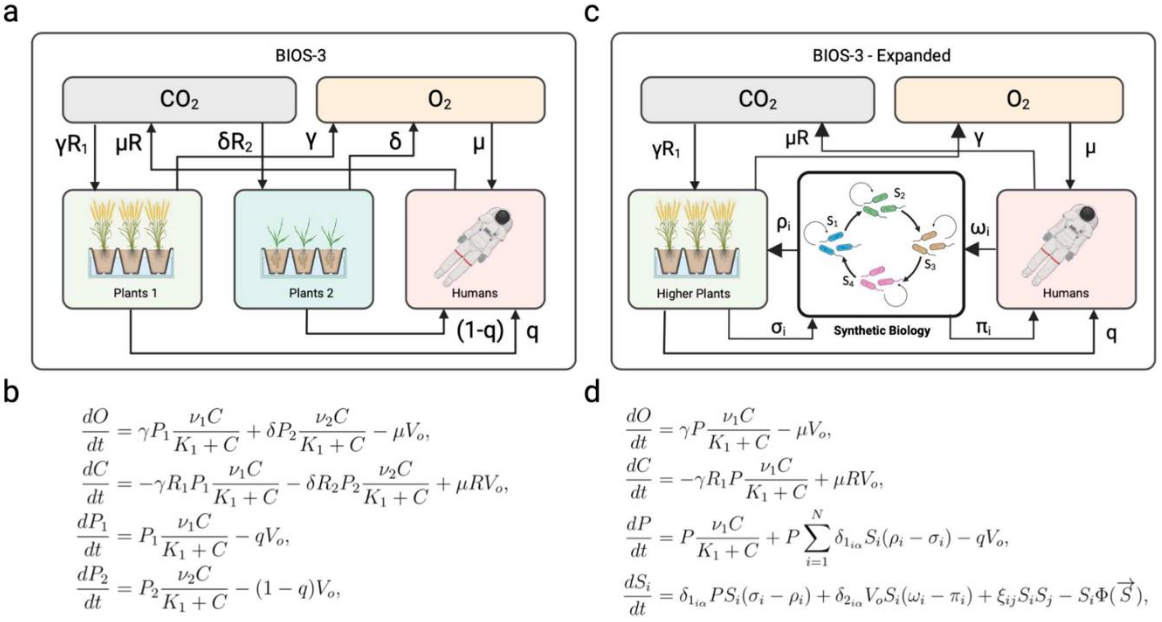
\includegraphics[width=0.8\textwidth]{figs/bios-3_schemes.png}
%	\end{figure}
%}


%%%%%%%%%%%%%%%%%%%%%%%%%%%%%%%%%%%%%%%%%%%%%%%%%%%%%%%%%%%%%%%%%%
%% Caffeine intake
%%%%%%%%%%%%%%%%%%%%%%%%%%%%%%%%%%%%%%%%%%%%%%%%%%%%%%%%%%%%%%%%%%


\frame{
	\frametitle{Caffeine intake}
	Coffee to the rescue!
	\begin{figure}
		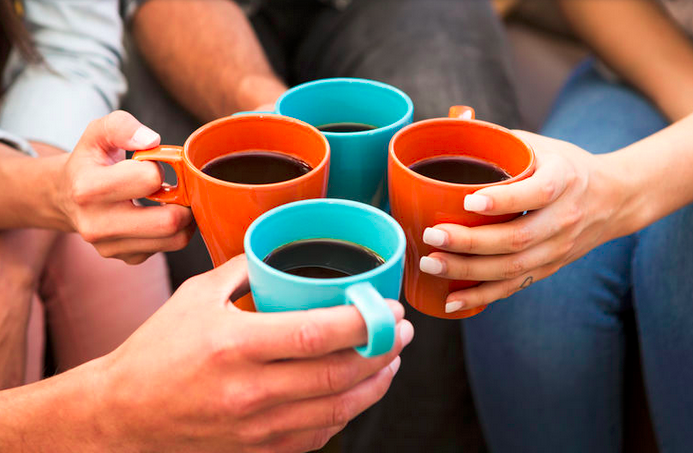
\includegraphics[width=0.7\textwidth]{figs/caffeine_intake_coffee.png}
	\end{figure}
}


\frame{
	\frametitle{Caffeine intake}
	
	\begin{itemize}
	\item Simple pharmacodynamics model:
	\begin{itemize}
	\item absorption of caffeine
	\item removal of caffeine
	\item stimulating effect (Hill-function)
	\end{itemize}		
	\item ODEs / Bayesian modeling
	\item Optimization/sampling of good caffeine dosing schedules
	\item Individualizing caffeine dosing strategies, based on:
	\begin{itemize}
	\item age
	\item genetics
	\item metabolism
	\end{itemize}
	\end{itemize}
}


%\frame{
%	\frametitle{Caffeine intake}
%
%\begin{figure}[H]
% \begin{minipage}{0.5\linewidth}
%  \centering
%  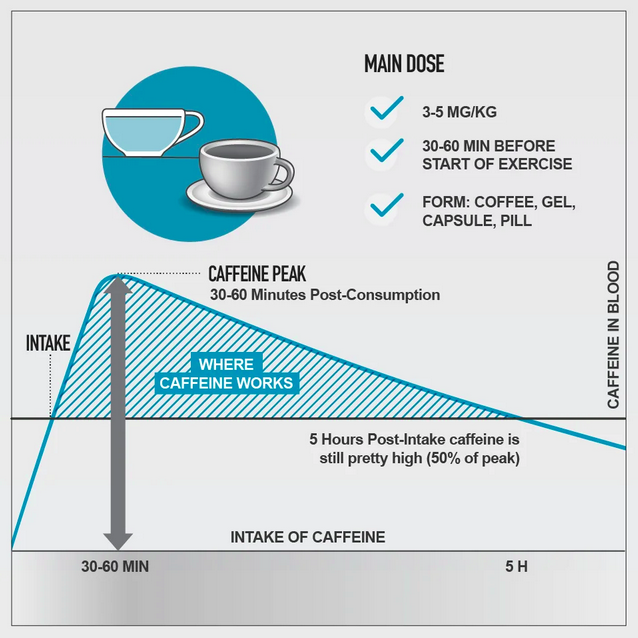
\includegraphics[width=0.8\textwidth]{figs/caffeine_intake_01.png}
% \end{minipage}%
% \begin{minipage}{0.5\linewidth}
%  \centering
%  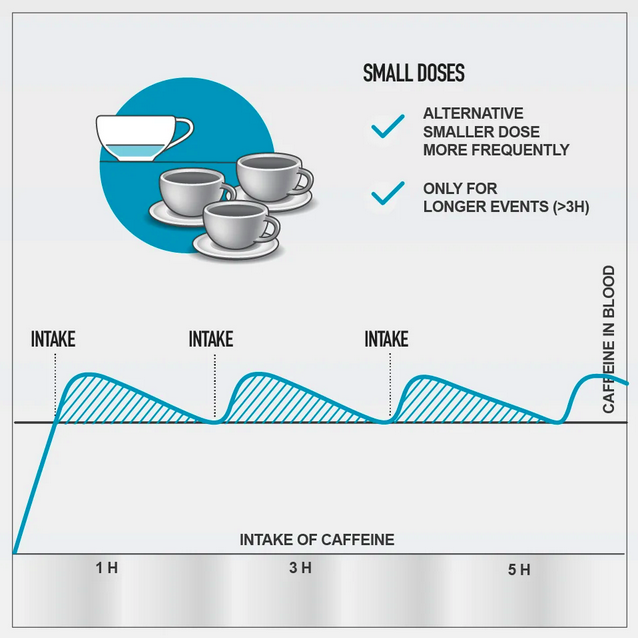
\includegraphics[width=0.8\textwidth]{figs/caffeine_intake_02.png}
% \end{minipage}
%\end{figure} 
%}

%%%%%%%%%%%%%%%%%%%%%%%%%%%%%%%%%%%%%%%%%%%%%%%%%%%%%%%%%%%%%%%%%%
%% LSD
%%%%%%%%%%%%%%%%%%%%%%%%%%%%%%%%%%%%%%%%%%%%%%%%%%%%%%%%%%%%%%%%%%


\frame{
	\frametitle{LSD}
	Effect of psychedelic drugs.
	\begin{figure}
		
\includegraphics[width=0.7\textwidth]{figs/lsd_tongue.png}
	\end{figure}

}


\frame{
	\frametitle{LSD}
	\begin{itemize}
	\item Develop ODE model based on two-compartment model
	\item Include more compartments or physiological details
	\item Incorporate different administration routes
	\item Analyze the behaviour of different doses and administration routes
	\item Impact of physiological parameters
	\item Role of metabolism and elimination processes
	\item Either estimate model parameters, do a sensitivity analysis, compare different model structures, explore inter-individual variability...
	\end{itemize}
}



%%%%%%%%%%%%%%%%%%%%%%%%%%%%%%%%%%%%%%%%%%%%%%%%%%%%%%%%%%%%%%%%%%
%% Defrosting seafood
%%%%%%%%%%%%%%%%%%%%%%%%%%%%%%%%%%%%%%%%%%%%%%%%%%%%%%%%%%%%%%%%%%


\frame{
	\frametitle{Defrosting seafood}
	Food safety aspects of thawing frozen seafood.
	\begin{figure}
		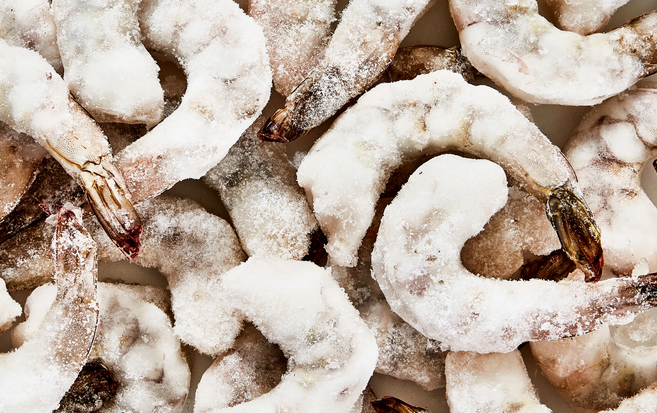
\includegraphics[width=0.8\textwidth]{figs/thawing_frozen_shrimps.png}
	\end{figure}
}


\frame{
	\frametitle{Defrosting seafood}
	\begin{itemize}
	\item Model this system as: ODE, SDE or SSA
	\item Interactive decision-support tool for risk of microbial spoilage
	\item Bayesian inference to estimate the parameters
	\item Explore different thawing strategies
	\item Effects of preparing or heating
	\item Uncertainty and sensitivity 
	\end{itemize}
}


%\frame{
%	\frametitle{Defrosting seafood}
%	\begin{figure}
%		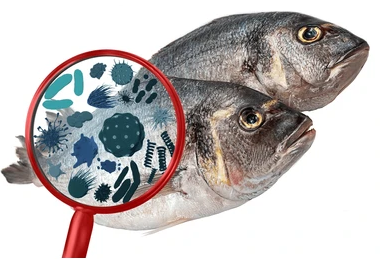
\includegraphics[width=0.8\textwidth]{figs/microbial_spoilage.png}
%	\end{figure}
%}


%%%%%%%%%%%%%%%%%%%%%%%%%%%%%%%%%%%%%%%%%%%%%%%%%%%%%%%%%%%%%%%%%%
%% Evolution of Virulence
%%%%%%%%%%%%%%%%%%%%%%%%%%%%%%%%%%%%%%%%%%%%%%%%%%%%%%%%%%%%%%%%%%


\frame{
	\frametitle{Evolution of Virulence}
	\begin{figure}
		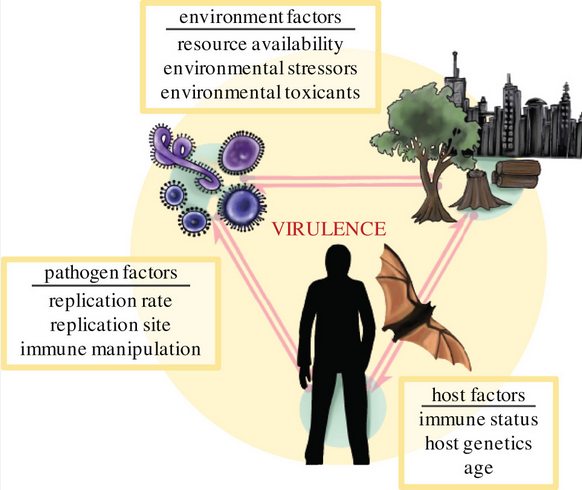
\includegraphics[width=0.7\textwidth]{figs/virulence_evolution.png}
	\end{figure}
}


\frame{
	\frametitle{Evolution of Virulence}
	\begin{itemize}
	\item Start from SIR model and incorporate virulence
	\item Consider different relationships between virulence and transmission
	\item Include multiple strains
	\item Explore competition/cooperation between strains and the overall effect on the evolution
	\item Variation in host susceptibility or resistance to infections
	\item Consider stochasticity
	\end{itemize}
}


%\frame{
%	\frametitle{Evolution of Virulence}
%	\begin{figure}
%		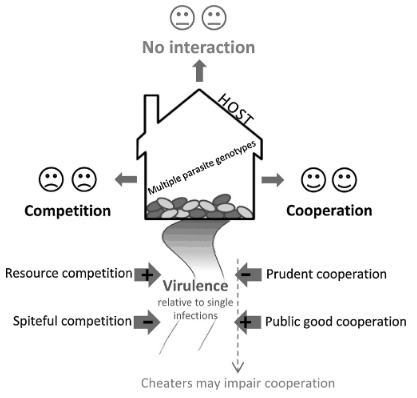
\includegraphics[width=0.6\textwidth]{figs/virulence_02.png}
%	\end{figure}
%}


\frame{
\frametitle{Interesting ideas to explore}

\begin{itemize}
	\item Sliders to study effects of changing parameters
	\item Sensitivity analysis to analyze parameter effect
	\item Monte Carlo simulation to incorporate uncertainty
	\item Stochasticity/sampling to include variation
	\item Optimize model parameters
	\item Validate with different data
	\item ...
\end{itemize}

\bigskip \pause

{\large
Use of \textbf{Generative AI} is allowed, e.g., \textit{NotebookLM}, \textit{Consensus}...
}

\bigskip \bigskip \centering

Have fun exploring!

\bigskip

}


\end{document}

